%%\title{Error Definitions}

\chapter{Error Definitions}
\label{chap:error}
This chapter describes the commands which provide error assignment and
output of errors assigned to elements. It is possible to assign
alignment errors and field errors to single beam elements or to ranges
or classes of beam elements.

Elements, classes or ranges of elements are selected by the
\hyperref[sec:select]{\texttt{SELECT}} command.

ATTENTION: since errors can only be assigned to machine elements, it is
necessary to \hyperref[sec:flatten]{\texttt{FLATTEN}} a sequence
if it includes other sequences.

Errors can be specified with both constant or random values.

Error definitions consist of four types of statements listed below. They
may be entered after having selected a beam line by means of a
\hyperref[sec:use]{\texttt{USE}} command.  

WARNING: any further \hyperref[sec:use]{\texttt{USE}} command
will destroy the assigned errors. Use the
\hyperref[sec:esave]{\texttt{ESAVE}} option to save and reload errors.

WARNING: if errors are to be applied to a thin sequence produced by \hyperref[chap:makethin]{\texttt{MAKETHIN}}, it is advisable to save the sequence on a file and then reload it, in order for \madx to reinitialize its data structures in a suitable way.

%\href{http://consult.cern.ch/xwho/people/1808}{Werner Herr} 18.6.2002 


%%%\title{EALIGN}
%  Changed by: Hans Grote, 13-Sep-2000 

%  Changed by: Werner Herr, 19-Jun-2002 

%  Changed by: Hans Grote, 19-Jun-2002 

%  Changed by: Werner Herr, 24-Jul-2002 

%  Changed by: Werner Herr, 02-Sep-2002 

%  Changed by: Hans Grote, 25-Sep-2002 

%%\usepackage{hyperref}
% commands generated by html2latex


%%\begin{document}

\section{EALIGN: Define Misalignments}  Alignment errors are defined by the EALIGN command. The misalignments refer to the \href{../Introduction/local_system.html}{local reference system} for a perfectly aligned machine. Possible misalignments are displacements along the three coordinate axes, and rotations about the coordinate axes. Alignment errors can be assigned to all beam elements except drift spaces. The effect of misalignments is treated in a linear approximation. A \href{read HREF=../Introduction/monitors.html}{Beam position monitor} can be given read errors in both horizontal and vertical planes. Monitor errors (MREX, MREY, MSCALX and MSCALY) are ignored for all other elements. Each new EALIGN statement replaces the misalignment errors for all elements in its range, unless EOPTION,ADD=TRUE has been entered. 

 Alignment errors are defined by the statement 
\begin{verbatim}

SELECT,FLAG=ERROR,RANGE=range,CLASS=name,PATTERN=string;
EALIGN, DX=real,DY=real,DS=real, 
        DPHI=real,DTHETA=real,DPSI=real, 
        MREX=real,MREY=real,
        MSCALX=real,MSCALY=real,
        AREX=real,AREY=real;
\end{verbatim} and elements are now selected by the \href{../Introduction/select.html}{SELECT} command. The attributes are: 

DX: The misalignment in the \textit{x}-direction for the entry of the beam element (default: 0 m). 
\\ DX$>$0 displaces the element in the positive \textit{x}-direction 

DY: The misalignment in the \textit{y}-direction for the entry of the beam element (default: 0 m). 
\\ DY$>$0 displaces the element in the positive \textit{y}-direction 

DS: The misalignment in the \textit{s}-direction for the entry of the beam element (default: 0 m). 
\\ DS$>$0 displaces the element in the positive \textit{s}-direction 

DPHI: The rotation around the \textit{x}-axis. 
\\ A positive angle gives a greater \textit{x}-coordinate for the exit than for the entry (default: 0 rad). 

DTHETA: The rotation around the \textit{y}-axis according to the right hand rule (default: 0 rad). 

DPSI: The rotation around the \textit{s}-axis according to the right hand rule (default: 0 rad). 

MREX: The horizontal read error for a monitor. This is ignored if the element is not a monitor 
\\ If MREX$>$0 the reading for \textit{x} is too high (default: 0 m). 

MREY: The vertical read error for a monitor. This is ignored if the element is not a monitor 
\\ If MREY$>$0, the reading for \textit{y} is too high (default: 0 m). 

AREX: The misalignment in the \textit{x}-direction for the entry of an aperture limit (default: 0 m). 
\\ AREX$>$0 displaces the element in the positive \textit{x}-direction 

AREY: The misalignment in the \textit{y}-direction for the entry of an aperture limit (default: 0 m). 
\\ AREY$>$0 displaces the element in the positive \textit{y}-direction 

MSCALX: The relative horizontal scaling error for a monitor. This is ignored if the element is not a monitor. 
\\ If MSCALX$>$0 the reading for \textit{x} is too high (default: 0). A value of 0.5 implies the actual reading is multiplied by 1.5. 

MSCALY: The relative vertical scaling error for a monitor. This is ignored if the element is not a monitor.  
\\ If MSCALY$>$0 the reading for \textit{y} is too high (default: 0). A value of -0.3 implies the actual reading is multiplied by 0.7. 
\\
\\
\\ Example: 
\begin{verbatim}

SELECT,FLAG=ERROR,CLASS=MQ;                  
EALIGN,DX=0.002,DY=0.0004*RANF(),DPHI=0.0002*GAUSS();
\end{verbatim} Assigns alignment errors to all elements of class MQ.           
\\
\begin{verbatim}

SELECT,FLAG=ERROR,PATTERN="QF.*";            
EALIGN,DX=0.001*TGAUSS(2.5),DY=0.0001*RANF();
\end{verbatim} Assigns alignment errors to all elements starting with "QF". TGAUSS(2.5) means a Gaussian distribution cut at 2.5 sigma. 
\\

%\href{xsdisp}{
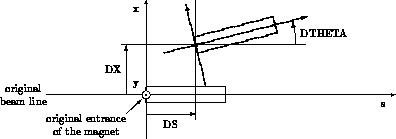
\includegraphics{figures/xs_align.png}

\textbf{Figure 1:} Example of Misplacement in the (\textit{x, s})-plane. 

%\href{xydisp}{
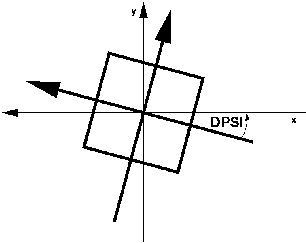
\includegraphics{error/dpsi.png}

\textbf{Figure 2:} Example of Misplacement in the (\textit{x, y})-plane. 

%\href{ysdisp}{
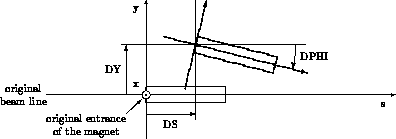
\includegraphics{figures/ys_align.png}

\textbf{Figure 3:} Example of Misplacement in the (\textit{y, s})-plane. 

%\href{monitor}{
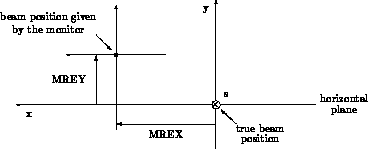
\includegraphics{figures/monitor_read.png}

\textbf{Figure 4:} Example of Read Errors in a monitor 
\\
\\
\\
\\\href{http://consult.cern.ch/xwho/people/1808}{Last updated:} 02.9.2002 \\\href{http://consult.cern.ch/xwho/people/1808}{Werner Herr} 18.6.2002 

%%\end{document}

%%\title{EALIGN}
%  Changed by: Hans Grote, 13-Sep-2000 
%  Changed by: Werner Herr, 19-Jun-2002 
%  Changed by: Hans Grote, 19-Jun-2002 
%  Changed by: Werner Herr, 24-Jul-2002 
%  Changed by: Werner Herr, 02-Sep-2002 
%  Changed by: Hans Grote, 25-Sep-2002 

\section{EALIGN: Alignment Errors and permanent misalignments} %EALIGN: Define Misalignments} 
\label{sec:ealign}

There are two ways of introducing misalignments in MAD-X.
\subsection{EALIGN}

Alignment errors are defined by the \texttt{EALIGN} command. 
The misalignments refer to the
\hyperref[sec:reference]{local reference system} for a
perfectly aligned machine.  
Misalignments are defined as displacements along the three coordinate
axes, and rotations about the coordinate axes. 
Alignment errors can be assigned to all beam elements except drift
spaces. 
The effect of misalignments is treated in a linear
approximation.

\hyperref[sec:monitor]{Beam Position Monitors} can be given readout errors as 
well as readout scaling errors in both horizontal and vertical planes. 
Monitor readout and scaling errors are ignored for all elements other than 
\hyperref[sec:monitor]{monitors}.

Each new \texttt{EALIGN} statement replaces the misalignment errors for all 
elements in its range, unless the logical \texttt{ADD} attribute of 
\hyperref[sec:eoption]{\texttt{EOPTION}} has been specified.

Alignment errors are defined by the statement 

\madbox{
xxxxxxxx\= \kill
SELECT, \>FLAG=ERROR, RANGE=range, CLASS=name, PATTERN=string; \\
EALIGN, \>DX=real, DY=real, DS=real, \\
        \>DPHI=real, DTHETA=real, DPSI=real,  \\
        \>MREX=real, MREY=real, \\
        \>MSCALX=real, MSCALY=real,\\
        \>AREX=real, AREY=real;
}
for elements selected by the
\hyperref[sec:select]{\texttt{SELECT}} command. 

\begin{figure}[ht]
	\centering
	\setlength{\unitlength}{1pt}
	\includegraphics{figures/f-xsdisp.pdf}
	\caption{Alignment errors in the $(x,s)$-plane}
	\label{F-XSDISP}
\end{figure}

\begin{figure}[htb]
	\centering
	\setlength{\unitlength}{1pt}
	\includegraphics{figures/f-xydisp.pdf}
	\caption{Alignment errors in the $(x,y)$-plane}
	\label{F-XYDISP}
\end{figure}

\subsection{Permanent Misalignments}
The second way of introducing misalignments in MAD-X is
to define them directly in the creation of a sequence. The name 
and effect of the orientation is the same as for the \texttt{EALIGN}. 
In case EALIGN and permanent misalignment are used togheter the values 
are added togheter component by component. The effect of the permanent misalignment
is ignored by SURVEY by default but by adding the \text{PERM\_ALIGN\_SURVEY} the 
start and end location of each element is given. The permanent misalignemnt need to 
be defined in the creation of the sequence. An example is given below:
\textbf{Examples:}
\madxmp{
a=0.06; \\
q1:quadrupole, l=1, k1=0.01; \\
myseq: sequence, l=10; \\
q1, at=5, dtheta=0.1, dphi=0.2, dpsi=0.3, dx=0.04, dy=0.05, ds:=a; \\
endsequence; \\
}
It is also possible to defined the permanet misalignments using defered expresions.
%% \begin{figure}[ht]
%% \centering
%% \setlength{\unitlength}{1pt}
%% \begin{picture}(400,140)(0,30)
%% \thinlines
%% \put(50,75){\line(1,0){96}}
%% \put(154,75){\vector(1,0){246}}
%% \put(50,75){\makebox(0,0)[r]{\shortstack{original \\beam line}}}
%% \put(390,65){\makebox(0,0)[r]{s}}
%% \put(150,75){\circle{8}}
%% \put(150,75){\circle*{2}}
%% \put(140,85){\makebox(0,0){x}}
%% \put(150,30){\line(0,1){41}}
%% \put(150,79){\vector(0,1){91}}
%% \put(140,160){\makebox(0,0){y}}
%% \put(130,55){\vector(1,1){15}}
%% \put(130,55){\makebox(0,0)[tr]{\shortstack{original entrance \\
%% of the magnet}}}
%% \thicklines
%% \put(150,55){\vector(1,0){50}}
%% \put(175,45){\makebox(0,0){DS}}
%% \put(130,75){\vector(0,1){50}}
%% \put(125,100){\makebox(0,0)[r]{DY}}
%% \thinlines
%% \put(125,125){\line(1,0){185}}
%% \put(200,50){\line(0,1){120}}
%% \put(200,125){\circle*{4}}
%% \thicklines
%% \put(168,133){\vector(4,-1){144}}
%% \put(189,81){\vector(1,4){22}}
%% \bezier{30}(300,125)(300,113)(297,101)
%% \put(299,109){\vector(-1,-4){2}}
%% \put(305,113){\makebox(0,0)[l]{DPHI}}
%% \put(278,97){\line(1,4){4}}
%% \put(198,117){\line(1,4){4}}
%% \put(202,133){\line(4,-1){80}}
%% \put(198,117){\line(4,-1){80}}
%% \put(150,67){\line(1,0){80}}
%% \put(150,83){\line(1,0){80}}
%% \put(150,67){\line(0,1){4}}
%% \put(150,79){\line(0,1){4}}
%% \put(230,67){\line(0,1){16}}
%% \end{picture}
%% \caption{Example of Misplacement in the $(y,s)$-plane (WRONG)}
%% \label{F-YSDISP}
%% \end{figure}

\begin{figure}[ht]
	\centering
	\setlength{\unitlength}{1pt}
	\includegraphics{figures/f-ysdisp.pdf}
	\caption{Alignment errors in the $(y,s)$-plane}
	\label{F-YSDISP}
\end{figure}

The attributes are: 
\begin{madlist}
  \ttitem{DX} The misalignment in the \textit{x}-direction for the entry of
  the beam element. (Default:~0~m).  \\ 
  \texttt{DX}$>$0 displaces the element in the positive \textit{x}-direction 
  
  \ttitem{DY} The misalignment in the \textit{y}-direction for the entry of
  the beam element. (Default:~0~m). \\
  \texttt{DY}$>$0 displaces the element in the positive \textit{y}-direction 

  \ttitem{DS} The misalignment in the \textit{s}-direction for the entry of
  the beam element. (Default:~0~m). \\
  \texttt{DS}$>$0 displaces the element in the positive \textit{s}-direction 
  
  \ttitem{DPHI} The rotation around the \textit{x}-axis. (Default:~0~rad). \\ 
  A positive angle gives a greater \textit{y}-coordinate for the exit
  than for the entry. 

  \ttitem{DTHETA} The rotation around the \textit{y}-axis according to the
  right hand rule. (Default:~0~rad).  

  \ttitem{DPSI} The rotation around the \textit{s}-axis according to the
  right hand rule. (Default:~0~rad).  

  \ttitem{MREX} The horizontal read error for a monitor. This is ignored if
  the element is not a monitor. Note that this is ignored by TWISS and TRACK
  and only used by the orbit correction command.  \\
  If \texttt{MREX}$>$0 the reading for \textit{x} is too high (default: 0 m). 

  \ttitem{MREY} The vertical read error for a monitor. This is ignored if
  the element is not a monitor. Note that this is ignored by TWISS and TRACK
  and only used by the orbit correction command.  \\  
  If \texttt{MREY}$>$0, the reading for \textit{y} is too high (default: 0 m). 

  \ttitem{MSCALX} The relative horizontal scaling error for a monitor. This
  is ignored if the element is not a monitor. Note that this is ignored by TWISS and TRACK
  and only used by the orbit correction command.  \\ 
  If \texttt{MSCALX}$>$0 the reading for \textit{x} is too high (default: 0). A
  value of 0.5 implies that the actual reading is multiplied by 1.5.  

  \ttitem{MSCALY} The relative vertical scaling error for a monitor. This is
  ignored if the element is not a monitor. Note that this is ignored by TWISS and TRACK
  and only used by the orbit correction command.  \\ 
  If \texttt{MSCALY}$>$0 the reading for \textit{y} is too high (default: 0). A
  value of -0.3 implies that the actual reading is multiplied by 0.7.  

  \ttitem{AREX} The misalignment in the \textit{x}-direction for the entry
  of an aperture limit (default: 0 m). \\ 
  \texttt{AREX}$>$0 displaces the element in the positive \textit{x}-direction 

  \ttitem{AREY} The misalignment in the \textit{y}-direction for the entry
  of an aperture limit (default: 0 m). \\ 
  \texttt{AREY}$>$0 displaces the element in the positive \textit{y}-direction 

\end{madlist}

\begin{figure}[htb]
	\centering
	\setlength{\unitlength}{1pt}
	\includegraphics{figures/f-ermoni.pdf}
	\caption{Readout errors in a monitor}
	\label{F-ERMONI}
\end{figure}

\textbf{Examples:}
\madxmp{
SELECT, FLAG = ERROR, CLASS = MQ; \\
EALIGN, DX = 0.002, DY = 0.0004*RANF(), DPHI = 0.0002*GAUSS();
}
Assigns alignment errors to all elements of class \texttt{MQ}.

\madxmp{
SELECT, FLAG = ERROR, PATTERN = "QF.*"; \\
EALIGN, DX = 0.001*TGAUSS(2.5), DY = 0.0001*RANF();
}
Assigns alignment errors to all elements starting with \texttt{"QF"}. \texttt{
TGAUSS(2.5)} specifies a Gaussian distribution cut at 2.5 sigma.

%\href{http://consult.cern.ch/xwho/people/1808} {Last updated:} 02.9.2002 \\ 
%\href{http://consult.cern.ch/xwho/people/1808}{Werner Herr} 18.6.2002 

%%%\title{Field Errors}
%  Changed by: Hans Grote, 19-Jun-2002 

\section{Field Errors}
Field errors can be entered as relative or absolute errors. Different
multipole components can be specified with different kinds of errors
(relative or absolute). Relations between absolute and relative field
errors are listed below.  

In MAD8 two commands were used for that purpose: EFIELD and EFCOMP. Only
EFCOMP was implemented in MAD-X since it provides the full functionality
of EFIELD and there was no need for duplication.  

All field errors are specified as the integrated value
int(\textit{K*ds}) of the \href{../Introduction/sign_convent.html}{field
  components} along the magnet axis in m$^{-i}$. There is no provision
to specify a global relative excitation error affecting all field
components in a combined function magnet. Such an error may only be
entered by defining the same relative error for all field components.  

Field errors can be specified for all magnetic elements by the statement  

\begin{verbatim}
SELECT, FLAG = ERROR, RANGE = range, CLASS = name, PATTERN = string;
EFCOMP, ORDER := integer, RADIUS := real,
        DKN  := {dkn(0), dkn(1), dkn(2),...},
        DKS  := {dks(0), dks(1), dks(2),...},
        DKNR := {dknr(0),dknr(1),dknr(2),...},
        DKSR := {dksr(0),dksr(1),dksr(2),...};
\end{verbatim}
and elements are now selected by the
\href{../Introduction/select.html}{SELECT} command. Each new
\href{efcomp}{EFCOMP} statement replaces the field errors for all
elements in its range (s). Any old field errors present in the range are
discarded or incremented depending on the setting of
\href{error_option.html}{EOPTION,ADD}. EFCOMP defines them in terms of
relative or absolute components.  

The attributes are: 
\begin{itemize}
\item ORDER: If relative errors are entered for multipoles, this defines
  the order of the base component to which the relative  errors
  refer. This reference strength \textit{k$_ref$} always refers to the
  normal component. To use a skew component as the reference the
  reference radius should be specified as a negative number. The default
  is zero.  \\
  Please note that this implies to specify \textit{k$_0$} to assign
  relative field errors to a bending magnet since \textit{k$_0$} is used
  for the normalization and NOT the ANGLE.  

\item RADIUS: Radius \textit{R} were dknr(i) or dksr(i) are specified
  for 0...i...20 (default 1 m). This attribute is required if dknr(i) or
  dksr(i) are specified. If \textit{R} is negativ, the skew component is
  used for the reference strength.  

\item DKN(i): Absolute error for the normal multipole strength with
  (2i+2) poles (default: 0  m$^{-i}$).  

\item DKS(i): Absolute error for the skewed multipole strength with
  (2i+2) poles (default: 0  m$^{-i}$).  

\item DKNR(i): Relative error for the normal multipole strength with
  (2i+2) poles (default: 0  m$^{-i}$).  

\item DKSR(i): Relative error for the skewed multipole strength with
  (2i+2) poles (default: 0  m$^{-i}$).  
\end{itemize}


\subsection{Time memory effects:}

The relative errors can be corrected for possible time memory effects. A
correction term is computed and added to the relative error. 

The correction term is parametrized as a 3rd order polynomial in the
reference strength \textit{k$_ref$} according to:  

%\begin{verbatim}
\[ \Delta = \sum (c_i * \textit{k}^{i}_{ref})            i = 0...3\]
%\end{verbatim}
The coefficients c$_i$ for the polynominal must be supplied in the
command.  

Two additional parameters and options are required: 

HYSTER: if it is set to 1 applies the correction term derived from the
reference strength and the coefficients.  

HCOEFFN and HCOEFFS: coefficients (normal and skew) for the computation
of the correction term. The 4 coefficients are specified in increasing
order, starting with the 0th order. Each group of four coefficients is
valid for one order of the field errors. Trailing zeros can be omitted,
preceding zeros must be given.  

\subsection{Examples} 

Example 1 (assign relative errors to quadrupoles); 
\begin{verbatim}
select, flag = error, pattern = "q.*";
efcomp, order := 1, radius := 0.010,
dknr := {0, 4e-1, 1e-1, 2e-3, 0, 0, 0, 0, 0, 0, 0, 0, 0, 0, 0, 0, 0, 0, 0, 0},
dksr := {0, 4e-1, 1e-1, 2e-3, 0, 0, 0, 0, 0, 0, 0, 0, 0, 0, 0, 0, 0, 0, 0, 0};
\end{verbatim}

Example 2 (add time memory effect to relative errors): 
\begin{verbatim}
select, flag = error, pattern = "^q.*";
efcomp, order = 1, radius = 0.020, hyster = 1,
hcoeffn := {0.000, 0.000, 0.000, 0.000,   // coefficients multipole order 0
            0.001, 0.000, 0.000, 0.000,   // coefficients multipole order 1
            0.000, 0.000, 0.002, 0.000},  // coefficients multipole order 2
dknr := {0, 1e-2, 2e-4, 4e-5, 1e-5, 0, 0, 0, 0, 0, 0, 0, 0, 0, 0, 0, 0, 0, 0, 0},
dksr := {0, 1e-2, 2e-4, 4e-5, 1e-5, 0, 0, 0, 0, 0, 0, 0, 0, 0, 0, 0, 0, 0, 0, 0};
\end{verbatim}

See also: \href{../Introduction/expression.html#random}{Random values}
and \href{../Introduction/expression.html#defer}{deferred expressions}.  

%\href{http://consult.cern.ch/xwho/people/1808}{Werner Herr}  6.12.2004 

%%\title{Field Errors}
%  Changed by: Hans Grote, 19-Jun-2002 

\section{EFCOMP: Field Errors}
\label{sec:efcomp}
Field errors can be entered as relative or absolute errors. Different
multipole components can be specified with different kinds of errors
(relative or absolute). Relations between absolute and relative field
errors are listed below.  

In \madeight two commands were used for that purpose: \texttt{EFIELD} 
and \texttt{EFCOMP}.
Only \texttt{EFCOMP} was implemented in \madx since it provides the full 
functionality
of \texttt{EFIELD} and there was no need for duplication.  

All field errors are specified as the integrated value $\int K ds$ 
of the \hyperref[sec:sign-convention]{field components} along the magnet axis 
in $m^{-i}$. There is no provision
to specify a global relative excitation error affecting all field
components in a combined function magnet. Such an error may only be
entered by defining the same relative error for all field components.  

Field errors can be specified for all magnetic elements by the statement  

%% \begin{verbatim}
%% SELECT, FLAG = ERROR, RANGE = range, CLASS = name, PATTERN = string;
%% EFCOMP, ORDER := integer, RADIUS := real,
%%         DKN  := {dkn(0), dkn(1), dkn(2),...},
%%         DKS  := {dks(0), dks(1), dks(2),...},
%%         DKNR := {dknr(0),dknr(1),dknr(2),...},
%%         DKSR := {dksr(0),dksr(1),dksr(2),...};
%% \end{verbatim}

\madbox{
xxxxxxxx\=xxxxxx\= \kill
SELECT, \>FLAG=ERROR, RANGE=range, CLASS=name, PATTERN=string; \\
EFCOMP, \>ORDER=integer, RADIUS=real, \\
xxxxxxxx\=xxxxxx\=xxxxxxxxxx\=xxxxxxxxx\= \kill
        \>DKN= \>\{dkn(0),  \>dkn(1),  \>dkn(2),\ldots\}, \\
        \>DKS= \>\{dks(0),  \>dks(1),  \>dks(2),\ldots\}, \\
        \>DKNR=\>\{dknr(0), \>dknr(1), \>dknr(2),\ldots\}, \\
        \>DKSR=\>\{dksr(0), \>dksr(1), \>dksr(2),\ldots\};
}
for elements selected by the
\hyperref[sec:select]{\texttt{SELECT}} command.

Each new \texttt{EFCOMP} statement replaces the field errors for all
elements in its range(s). Previous field errors present in the range are
discarded or incremented depending on the setting of
\texttt{ADD} logical attribute of the
\hyperref[sec:eoption]{\texttt{EOPTION}} command. 
\texttt{EFCOMP} defines the field errors in terms of
relative or absolute components.

The attributes are: 
\begin{madlist}
  \ttitem{ORDER} If relative errors are entered for multipoles, this defines
  the order of the base component to which the relative  errors
  refer. This reference strength $k_{ref}$ always refers to the
  normal component. In order to use a skew component as the reference, the
  reference radius should be specified as a negative number. (Default:~0)  \\
  Please note that this implies to specify $k_0$ to assign
  relative field errors to a bending magnet since $k_0$ is used
  for the normalization and NOT the ANGLE. 

  \ttitem{RADIUS} radius \textit{R} where dknr(i) or dksr(i) are specified
  for 0...i...20 (default 1 m). This attribute is required if dknr(i) or
  dksr(i) are specified. If \textit{R} is negative, the skew component is
  used for the reference strength.  

  \ttitem{DKN(i)} Absolute error for the normal multipole strength with
  (2i+2) poles. (Default:~0~m$^{-i}$).  

  \ttitem{DKS(i)} Absolute error for the skewed multipole strength with
  (2i+2) poles. (Default:~0~m$^{-i}$).  

  \ttitem{DKNR(i)} Relative error for the normal multipole strength with
  (2i+2) poles. (Default:~0). The absolute error is computed from \texttt{DKNR(i)} using the following formula
  $$\Delta K_{i}=\texttt{DKNR(i)}\cdot\left(k_{ref}\right)\cdot R^{n-j}\cdot\frac{j!}{n!}$$
  where $n$ is the order of the reference strength, $k_{ref}$, specified in \texttt{ORDER}, and $R$ is the \texttt{RADIUS}.

  \ttitem{DKSR(i)} Relative error for the skewed multipole strength with
  (2i+2) poles. (Default:~0). The absolute error is computed from \texttt{DKSR(i)} using the following formula
  $$\Delta K_{i}=\texttt{DKSR(i)}\cdot\left(k_{ref}\right)\cdot |R|^{n-j}\cdot\frac{j!}{n!}$$
  where $n$ is the order of the reference strength, $k_{ref}$, specified in \texttt{ORDER}, and $R$ is the \texttt{RADIUS}. 
\end{madlist}

 Please note that even though that any order of field errors can be specified 
 for all elements, only those which are defined for an element will be taken into account.
 Only \texttt{K0} and  \texttt{K1} are be considered for  \hyperref[sec:bend]{\texttt{BEND}} 
 transfer map, and, in addition, \texttt{K2} and \texttt{K1S} for radiation effect. Only 
 \texttt{K1} and \texttt{K1S} are considered for  \hyperref[sec:quadrupole]{\texttt{QUADRUPOLE}}; 
 \texttt{K2}  and \texttt{K2S} - for \hyperref[sec:sextupole]{\texttt{SEXTUPOLE}}. Only 
 \hyperref[sec:multipole]{\texttt{THIN MULTIPOLE}} considers the erros of all orders. 
 
\textbf{Time memory effects:}

The relative errors can be corrected for possible time memory effects. A
correction term is computed and added to the relative error. 

The correction term is parametrized as a 3rd order polynomial in the
reference strength $k_{ref}$ according to:  
\[ \Delta = \sum (c_i * {\mathit k}^{i}_{ref})            i = 0...3\]
The coefficients $c_i$ for the polynomial must be supplied in the
command.  

Two additional parameters and options are required: 
\begin{madlist}
  \ttitem{HYSTER} if it is set to 1 applies the correction term derived from the
  reference strength and the coefficients.  

  \ttitem{HCOEFFN, HCOEFFS} normal and skew coefficients for the computation
  of the correction term. The four coefficients are specified in increasing
  order, starting with the 0th order. Each group of four coefficients is
  valid for one order of the field errors. Trailing zeros can be omitted,
  preceding zeros must be given.  
\end{madlist}

\textbf{Examples:}

Example to assign relative errors to quadrupoles: 
%% \begin{verbatim}
%% select, flag = error, pattern = "q.*";
%% efcomp, order = 1, radius = 0.010,
%% dknr := {0, 4e-1, 1e-1, 2e-3, 0, 0, 0, 0, 0, 0, 0, 0, 0, 0, 0, 0, 0, 0, 0, 0},
%% dksr := {0, 4e-1, 1e-1, 2e-3, 0, 0, 0, 0, 0, 0, 0, 0, 0, 0, 0, 0, 0, 0, 0, 0};
%% \end{verbatim}
\madxmp{
xxxxxxxx\=xxxxxxx\= \kill
SELECT, FLAG=error, PATTERN="q.*"; \\
EFCOMP, \>ORDER=1, RADIUS=0.010, \\
        \>DKNR=\{\>0, 4e-1, 1e-1, 2e-3, 0, 0, 0, 0, 0, 0, \\
        \>       \>0, 0, 0, 0, 0, 0, 0, 0, 0, 0\}, \\
        \>DKSR=\{\>0, 4e-1, 1e-1, 2e-3, 0, 0, 0, 0, 0, 0, \\
        \>       \>0, 0, 0, 0, 0, 0, 0, 0, 0, 0\};
}


Example to add time memory effect to relative errors: 
%% \begin{verbatim}
%% select, flag = error, pattern = "^q.*";
%% efcomp, order = 1, radius = 0.020, hyster = 1,
%% hcoeffn := {0.000, 0.000, 0.000, 0.000,   // coefficients multipole order 0
%%             0.001, 0.000, 0.000, 0.000,   // coefficients multipole order 1
%%             0.000, 0.000, 0.002, 0.000},  // coefficients multipole order 2
%% dknr := {0, 1e-2, 2e-4, 4e-5, 1e-5, 0, 0, 0, 0, 0, 0, 0, 0, 0, 0, 0, 0, 0, 0, 0},
%% dksr := {0, 1e-2, 2e-4, 4e-5, 1e-5, 0, 0, 0, 0, 0, 0, 0, 0, 0, 0, 0, 0, 0, 0, 0};
%% \end{verbatim}
\madxmp{
xxxxxxxx\=xxxxxxx\= \kill
SELECT, \>FLAG=error, PATTER="\^ q.*"; [FIXME] \\ 
EFCOMP, \>ORDER=1, RADIUS=0.020, HYSTER=1, \\
        \>DKNR=\{\>0, 1e-2, 2e-4, 4e-5, 1.e-5, 0, 0, 0, 0, 0, \\
        \>       \>0, 0, 0, 0, 0, 0, 0, 0, 0, 0\}, \\
        \>DKSR=\{\>0, 1e-2, 2e-4, 4e-5, 1.e-5, 0, 0, 0, 0, 0, \\
        \>       \>0, 0, 0, 0, 0, 0, 0, 0, 0, 0\}, \\
xxxxxxxx\=xxxxxxxxx\=xxxxxxxxxxxxxxxxxxxxxxxxxxxxx\= \kill
        \>HCOEFFN=\{\>0.000, 0.000, 0.000, 0.000, \>! coeff. mult. order 0 \\
        \>          \>0.001, 0.000, 0.000, 0.000, \>! coeff. mult. order 1 \\
        \>          \>0.000, 0.000, 0.002, 0.000\};\>! coeff. mult. order 2
}

See also: \hyperref[subsubsec:random]{random values}
and \hyperref[sec:defer]{deferred expressions}.  

%\href{http://consult.cern.ch/xwho/people/1808}{Werner Herr}  6.12.2004 


%%%\title{EOPTION}
%  Changed by: Hans Grote, 13-Sep-2000 

%  Changed by: Werner Herr, 19-Jun-2002 

%%\usepackage{hyperref}
% commands generated by html2latex


%%\begin{document}

\section{EOPTION: Set Error Options}  The random generator for MAD is taken from \href{../Introduction/bibliography.html#knuth}{[Knuth]}. The error option command specifies different seeds for random values: 
\begin{verbatim}

EOPTION,SEED=real,ADD=logical;
\end{verbatim}
\begin{itemize}
	\item SEED: Selects a particular sequence of random values. A SEED value is an integer in the range [0...999999999] (default: 123456789). SEED alone continues with the current sequence See also: \href{../Introduction/expression.html#random}{Random values}. SEED may be an expression. 
	\item ADD: If this logical flag is set, an EALIGN or EFCOMP, causes the errors to be added on top of existing ones. If it is not set, new errors overwrite any previous definitions. The default value is TRUE if it is omitted in the EOPTION command. The default value is false if no EOPTION command is used. 
\\Please note a recent modification: the default value for the ADD option is only applied as long as the ADD option has not been set explicitly.
\\ Once it was set with EOPTION, it is NOT reset to the default when       the ADD option is omitted in subsequent calls to EOPTION. 
\end{itemize} Example: 
\begin{verbatim}

EOPTION,SEED=987456321;
\end{verbatim}\href{http://consult.cern.ch/xwho/people/1808}{Werner Herr} 18.6.2002 

%%\end{document}

%%\title{EOPTION}
%  Changed by: Hans Grote, 13-Sep-2000 
%  Changed by: Werner Herr, 19-Jun-2002 

\section{EOPTION: Set Options for Error Definition} %EOPTION: Set Error Options}
\label{sec:eoption}
The error option command specifies different seeds for random values:  

\vspace{2mm}
\madbox{
EOPTION, SEED=real, ADD=logical;
}\vspace{5mm}

\begin{madlist}
  \ttitem{SEED} Selects a particular sequence of random values. 
  A \texttt{SEED} value is an integer in the range [0...999999999] (default:
  123456789). Note that the seed set with this command is shared with the \hyperref[sec:track]{\texttt{TRACK}} and \hyperref[sec:coption]{\texttt{COPTION}} commands. See
  also: \hyperref[subsubsec:random]{Random Values}. 

  \ttitem{ADD} If this logical flag is set, an \texttt{EALIGN} or \texttt{EFCOMP} 
  causes the errors to be added on top of existing ones. If it is not set,
  new errors overwrite any previous definitions. The default value is
  TRUE if it is omitted in the \texttt{EOPTION} command. The default value is
  false if no \texttt{EOPTION} command is used.  
  \\Please note a recent modification: the default value for the ADD
  option is only applied as long as the ADD option has not been set
  explicitly. 
  \\Once it was set with \texttt{EOPTION}, it is NOT reset to the default when
  the \texttt{ADD} option is omitted in subsequent calls to \texttt{EOPTION}.  
\end{madlist}

Example: 
\madxmp{EOPTION, SEED = 987456321;}

The random number generator for \madx is taken from
\cite{knuth1981}. 


%%%\title{EPRINT}
%  Changed by: Hans Grote, 13-Sep-2000 

\section{EPRINT: List Machine Imperfections}  
\label{sec:eprint}
This command prints a table of errors assigned to elements. The range
for these elements has to be specified. Field errors are printed as
absolute errors, because all relative errors are transformed to the
corresponding absolute error at definition time. An error print is
requested by the statement  

\begin{verbatim}
SELECT, FLAG=ERROR, RANGE=range, CLASS=name, PATTERN=string;
EPRINT;
\end{verbatim}
and elements are now selected by the
\href{../Introduction/select.html}{SELECT} command.  


A listing for ALL elements, i.e. not only the selected, can be obtained
with the command  
\begin{verbatim}
EPRINT, FULL=TRUE;
\end{verbatim} 
In that case, the SELECT command has no effect.

% \href{http://consult.cern.ch/xwho/people/1808}{Werner Herr} 18.6.2002 

%\href{http://consult.cern.ch/xwho/people/1808}{Werner Herr} 18.6.2002 
%%\title{EPRINT}
%  Changed by: Hans Grote, 13-Sep-2000 

\section{EPRINT: List Machine Imperfections}  
\label{sec:eprint}
This command prints a table of errors assigned to elements. The range
for these elements has to be specified. Field errors are printed as
absolute errors, because all relative errors are transformed to the
corresponding absolute error at definition time. An error print is
requested by the statement  

\madbox{
SELECT, FLAG=ERROR, RANGE=range, CLASS=name, PATTERN=string;\\
EPRINT;
}
and elements are now selected by the
\hyperref[sec:select]{\texttt{SELECT}} command.  

A listing for ALL elements, i.e. not only the selected, can be obtained
with the command  
\madbox{
EPRINT, FULL=TRUE;
}
In that case, the \texttt{SELECT} command has no effect.

% \href{http://consult.cern.ch/xwho/people/1808}{Werner Herr} 18.6.2002 

%%%\title{ESAVE}
%  Changed by: Hans Grote, 13-Sep-2000 
%  Changed by: Werner Herr, 19-Jun-2002 
%  Changed by: Hans Grote, 30-Sep-2002 

\section{Saving and reloading errors to and from tables and files} 
% ESAVE: Save Machine Imperfections and read back from file}

\subsection{Writing errors to a file}

\begin{verbatim}
ESAVE, FILE=string;
\end{verbatim}

This command saves a table of errors assigned to elements on a file,
using a format which can be read in again to obtain the same
results. This allows dumping the errors and reloading them after a new
USE command. The range for these elements has to be specified. An error
save is requested by the statement  

Example: 
\begin{verbatim}
SELECT, FLAG=ERROR, RANGE=range, CLASS=name, PATTERN=string;
ESAVE, FILE=err.file;
\end{verbatim} 
and elements selected by the  \href{../Introduction/select.html}{SELECT}
command are saved to the file.  


To save the errors of all elements to a file, one can use: 
\begin{verbatim}
SELECT, FLAG = ERROR, FULL;                                    
ESAVE, FILE = err.file;
\end{verbatim}

{\bf Please note: in case of field errors, the absolute errors are
  saved and not relative errors. } 

\subsection{Reading errors from a table or file}

To assign errors from a file is not a priori straightforward. It may be
required to re-assign existing errors after a \textbf{USE} command was
executed (which deletes all errors attached to a sequence).  

Errors stored in the form of an internal table (\textit{errtab}) can  be
directly attached to the appropriate positions in the sequence with the
command:  

\begin{verbatim}
SETERR, TABLE=errtab;
\end{verbatim}
The table \textit{errtab} can be generated internally or from an
external file (\textit{errfile}) with the generic command READMYTABLE.  
 

The command sequence: 
\begin{verbatim}
READMYTABLE, file=errfile, table=errtab;
SETERR, TABLE=errtab;
\end{verbatim}
reads the file \textit{errfile} into the table \textit{errtab} and the
command SETERR attaches the errors to the elements in the active
sequence.  

The file \textit{errfile} can be produced by a preceding ESAVE command
or any other utility. It should follow the format of a file generated
with ESAVE (see example program). 

{\bf Please note:}
\begin{enumerate}
   \item To assign correctly the errors from the file to the elements in
     the sequence, all elements must have individual names, otherwise an
     identification is not possible. Elements in the file not identified
     in the active sequence are ignored.  
   \item Errors are assigned to ALL elements found in the file and the
     FLAG=ERROR is set. Therefore the number of elements selected
     corresponding to a command like:  
     \\ SELECT, FLAG=ERROR,...;
     \\ can be different after the execution of SETERR. 
\end{enumerate}

%\href{http://consult.cern.ch/xwho/people/1808}{Werner Herr} 18.6.2002 


%%\title{ESAVE}
%  Changed by: Hans Grote, 13-Sep-2000 
%  Changed by: Werner Herr, 19-Jun-2002 
%  Changed by: Hans Grote, 30-Sep-2002 

% ESAVE: Save Machine Imperfections and read back from file}
\section{ESAVE: Writing errors to a file}
\label{sec:esave}

\madbox{
ESAVE, FILE=string;
}

This command saves a table of errors assigned to elements on a file,
using a format which can be read in again to obtain the same
results. This allows dumping the errors and reloading them after a new
USE command. The range for these elements has to be specified. An error
save is requested by the statement  

Example: 
\madxmp{
SELECT, FLAG=ERROR, RANGE=range, CLASS=name, PATTERN=string;
ESAVE, FILE=err.file;
}
and elements selected by the  \hyperref[sec:select]{\texttt{SELECT}}
command are saved to the file.  


To save the errors of all elements to a file, one can use: 
\madxmp{
SELECT, FLAG = ERROR, FULL; \\
ESAVE, FILE = err.file;
}

\textbf{Please note: in case of field errors, the absolute errors are
  saved and not relative errors. } 

\section{ETABLE: Saving the errors to a table}
\label{sec:esave}

\madbox{
ESAVE, TABLE=string;
}

This command saves a table of errors assigned to elements on a table,
using a format which can be read in again to obtain the same
results. This allows storing the errors and reloading them after a new
USE command. 

Example: 
\madxmp{
SELECT, FLAG=myerrortable, RANGE=range, CLASS=name, PATTERN=string; \\
ETABLE, TABLE=myerrortable;
}
and elements selected by the  \hyperref[sec:select]{\texttt{SELECT}}
command are stored to the table.  


\section{SETERR: Reading errors from a table or file}
\label{sec:seterr}

To assign errors from a file is not a priori straightforward. It may be
required to re-assign existing errors after a \hyperref[sec:use]{\texttt{USE}}
command was executed since the \texttt{USE} command deletes all errors attached to 
a sequence).

Errors stored in the form of an internal table (\textit{errtab}) can  be
directly attached to the appropriate positions in the sequence with the
command:  

\madbox{
SETERR, TABLE=errtab;
}

The table \textit{errtab} can be generated internally or from an
external file (\textit{errfile}) with the generic command \texttt{READTABLE}.
 

The command sequence: 
\madxmp{
READTABLE, file=errfile, table=errtab; \\
SETERR, TABLE=errtab;
}

reads the file \textit{errfile} into the table \textit{errtab} and the
command \texttt{SETERR} attaches the errors to the elements in the active
sequence.  

The file \textit{errfile} can be produced by a preceding \texttt{ESAVE} command
or any other utility. It should follow the format of a file generated
with \texttt{ESAVE} (see example program). 

\textbf{Please note:}
\begin{enumerate}
   \item To assign correctly the errors from the file to the elements in
     the sequence, all elements must have individual names, otherwise an
     identification is not possible. Elements in the file not identified
     in the active sequence are ignored.  
   \item Errors are assigned to ALL elements found in the file and the
     \texttt{FLAG=ERROR} is set. Therefore the number of elements selected
     corresponding to a command like
     \\ \texttt{SELECT, FLAG=ERROR,...;}
     \\ can be different after the execution of \texttt{SETERR}. 
\end{enumerate}

%\href{http://consult.cern.ch/xwho/people/1808}{Werner Herr} 18.6.2002 

%% EOF
